\section{Auslegung der Kupplung}
Im Folgenden wird die Sicherheitskupplung so ausgelegt, dass sie bei dem 1,5 fachen Wert des Momentes der Welle I durch rutscht. Dafür wird die Kraft berechnet, die auf die Kupplung durch zwei in Reihe geschaltete Tellerfedern aufgebracht werden muss. Anschließend wird der Weg berechnet, und den die Federn zusammengedrückt werden müssen, um die nötige Kraft aufzubringen. Bei der Sicherheitskupplung handelt es sich um eine Konuskupplung. Die verwendeten Formlen stammen aus dem Skript KL III \ccite{bib:poll:kl3} Seite 91 und 108 


\begin{align*}
	&M_{\mathrm{I},max} = 60,17 Nm \text{, } S = 1,5 \implies M = M_{\mathrm{I},max} \x S = 90,255 \text{ Nm} \\
	&\alpha = 20 ^\circ \text{, } \mu = 0,43 \text{ (siehe Abb. 2.1, Datenblatt)} \\
	&M = \mu \x \frac{F}{\sin\alpha} \x r_{eff} \\
	&r_{eff} = \frac{2}{3} \x \left( \frac{r_a^3- r_i^3}{r_a^2 - r_i ^2} \right) \text{ mit } r_a = 35 \text{ mm, } r_i = 31,57 \text{ mm} \\
	&\implies r_{eff} = 33,31 \text{ mm} \\
	&F = \frac{M \x \sin\alpha}{\mu \x r_{eff}} = 2155,16 \text{ N}
\end{align*}

Wähle zwei Tellerfedern nach DIN 2093 - B 40 \\
$ \implies F_{max} = 2,62 $ kN bei $ s_{max} = 0,86 $ mm (Tabellenbuch Metall \ccite{bib:fischer:tabellenbuchMetall} Seite 247)

\begin{align*}
	&c_{einzel} = \frac{F_{max}}{s_{max}} = 3,05 \frac{\text{kN}}{\text{mm}} \\
	&\frac{1}{c_{ges}} = 2 \x \frac{1}{c_{einzel}} \implies c_{ges} = 1,52 \frac{\text{kN}}{\text{mm}}\\
	&s = \frac{F}{c_{ges}} = \frac{2,1552 \text{ kN}}{1,52 \text{ kN/mm}} = 1,428 \text{ mm}
\end{align*}

	\begin{figure}[H]
		\vspace{-2cm}
		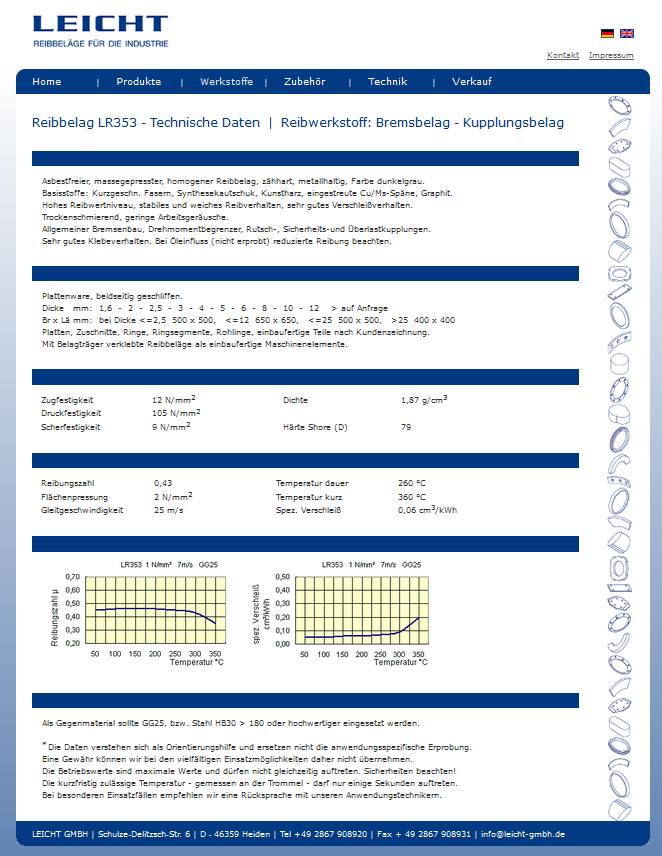
\includegraphics[width=1.0773\textwidth,keepaspectratio]{figures/Reibbelag.png}
		\caption{Datenblatt Reibbelag \protect\cite{bib:www:reibbelag}}
%		\caption{Datenblatt Reibbelag\protect\ccite{bib:www:reibbelag}\protect\footnotemark}
		\label{fig:Reibbelag}
	\end{figure}
	\footnotetext{Vgl. [Gmb] }